There exist two types of basic modules in \posl: \INTROom{} and \INTROopch{}. A \om{} is basically a function and a \opch{} is also a function, but in contrast, it can receive information from two different sources: through input parameters or from outside, i.e., by communicating with a module from another solver.

\subsection{Computation module}

%In this sub-section we expose the definition and the characteristics and the details of the \om, and give some examples. We explain how to create new \oms{} using the basic layer of the framework.

A \om{} is the most basic and abstract way to define a piece of computation. It is a function which receives an instance of a \posl{} data type as input, then executes an internal algorithm, and returns an instance of a \posl{} data type as output. The input and output types will characterize the computation module signature. It can be dy\-na\-mi\-cally replaced by (or combined with) other computation modules, since they can be transmitted to other solvers working in parallel. They are joined through operators defined in Section~\ref{sec:2ndstage}.

\defname{Computation Module}{
A \om{} $Cm$ is a mapping defined by: 
\begin{equation}
\label{def:om}
Cm:I \rightarrow O
\end{equation}
}

where $I$ and $O$, for instance, can be independently a set of configurations, a set of sets of configurations, a set of values of some data type, etc.

Consider a local search meta-heuristic solver. One of its \oms{} can be the function returning the set of configurations composing the neighborhood of a given configuration:

\begin{equation*}
Cm_{neighborhood}:I_1\times I_2\times\dots\times I_n \rightarrow 2^{I_1\times I_2\times\dots\times I_n}
\end{equation*}

\noindent where $I_i$ represents the definition domains of each variable of the input confi\-gura\-tion.

Figure~\ref{fig:om} shows an example of \om: which receives a configuration $S$ and then computes the set $\mathcal{V}$ of its neighbor configurations $\left\{S^1, S^2, \dots, S^m\right\}$.

%\vspace{0.5cm}
\begin{figure}
	\centering	
	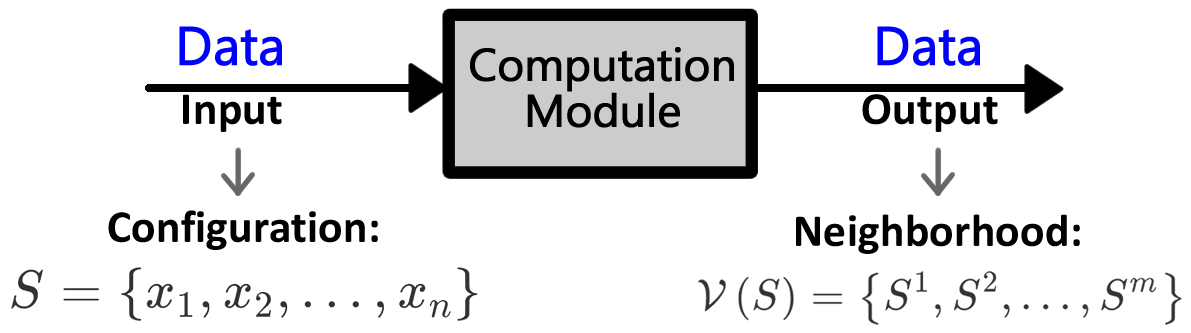
\includegraphics[width=0.7\linewidth]{OM.png}
	\caption{An example of a computation module computing a neighborhood}\label{fig:om}
\end{figure}

\subsubsection{Creating new \oms}
\label{subsubsec:creatingoms}

To create new \oms{} we use C++ programing language. \posl{} provides a hierarchy of data types to work with (see Appendix~\ref{app:diag}) and some abstract classes to inherit from, depending on the type of \om{} the user wants to create. These abstract classes represent {\it abstract} \oms{} and define a type of action to be executed. In the following we present the most important ones:

\begin{itemize}
\item \pclass{ACM\_FirstConfigurationGeneration} $\rightarrow$ Represents \oms{} returning a configuration, usually used for generating the starting configuration on local search meta-heuristics. The user must implement the method \pmethod{execute}{\pclass{ComputationData}} which returns a pointer to a \pclass{Solution}, that is, an object containing all the information concerning a partial solution (configuration, variable domains, etc.)
\item \pclass{ACM\_NeighborhoodFunction} $\rightarrow$ Represent \oms{} receiving a configuration as input and returning its neighborhood as output. The user must implement the method \pmethod{execute}{\pclass{Solution}} which returns a pointer to an object \pclass{Neighborhood}, containing a set of configurations which constitute the neighborhood of a given configuration, according to certain criteria. These configurations are efficiently stored in term of space.
\item \pclass{ACM\_SelectionFunction} $\rightarrow$ Represents \oms{} receiving a neighborhood as input and selecting a configuration from it as output. The user must implement the method \pmethod{execute}{\pclass{Neighborhood}} which returns a pointer to an object \pclass{DecisionPair}, containing two solutions: the current and the selected one.
\item \pclass{ACM\_DecisionFunction} $\rightarrow$ Represents \oms{} receiving a couple af configurations encapsulated into a \pclass{DecisionPair} object, and returning the configuration to be the current one for the next iteration. The user must implement the method \pmethod{execute}{\pclass{DecisionPair}} which returns a pointer to an object \pclass{Solution}.
\item \pclass{ACM\_ProcessingConfigurationFunction} $\rightarrow$ Represents \oms{} receiving a configuration and returning another configuration as result of some arrangement, like for example, a reset. The user must implement the method \pmethod{execute}{\pclass{Solution}} which returns a pointer to an object \pclass{Solution}.
\end{itemize}

\subsection{Communication modules}

%In this sub-section we expose the definition and the characteristics and the details of the \opch, and give some examples. We explain how to create new \opchs{} using the basic layer of the framework.

A \opch{} is the component managing the information reception in the communication between solvers (I talk about information transmission in Section~\ref{sec:2ndstage}). They can interact with \oms{} through operators (see Figure~\ref{fig:och}).

A \opch{} can receive two types of information from an external solver: data or \oms{}. It is important to notice that by sending/receiving \oms, I mean sending/receiving the required information to identify and being able to instantiate the \om. For instance, an integer identifier.

In order to distinguish from the two types of \opchs, I will call \INTROdopch{} the \opch{} responsible for the data reception (Figure~\ref{subfig:doch}), and \INTROoopch{} the one responsible for the reception and instantiation of \oms{} (Figure~\ref{subfig:ooch}).

\defname{Data Communication Module}{
A \emph{Data Communication Module} $Ch$ is a module that produces a mapping defined as follows: 
\begin{equation}
\label{def:dopench}
Ch:I\times \left\{D\cup \left\{NULL\right\}\right\} \rightarrow D \cup \left\{NULL\right\}
\end{equation}
No matter what the input $I$ is, it returns the information $D$ coming from an external solver.
}

\defname{Object Communication Module}{
	If we denote by $\mathbb{M}$ the space of all the \oms{} defined by Definition~\ref{def:om}, then an \emph{\oopch} $Ch$ is a module that produces and executes a \om{} coming from an external solver as follows:
	\begin{equation}
	\label{def:oopench}
	Ch:I\times\left\{\mathbb{M}\cup\left\{NULL\right\}\right\} \rightarrow O \cup \left\{NULL\right\}
	\end{equation}
It returns the output $O$ of the execution of the \om{} coming from an external solver, using $I$ as the input.
}%

\begin{figure}
	\centering
	\subfloat[][Data \opch]{
		\label{subfig:doch}
		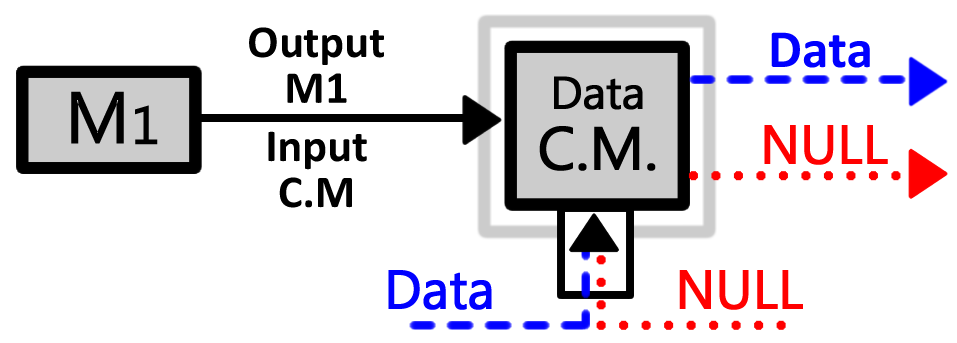
\includegraphics[width=0.4\linewidth]{D_OCh.png}
	}
	\hspace{0.05\textwidth}%
	\subfloat[][Object \opch]{%
		\label{subfig:ooch}
		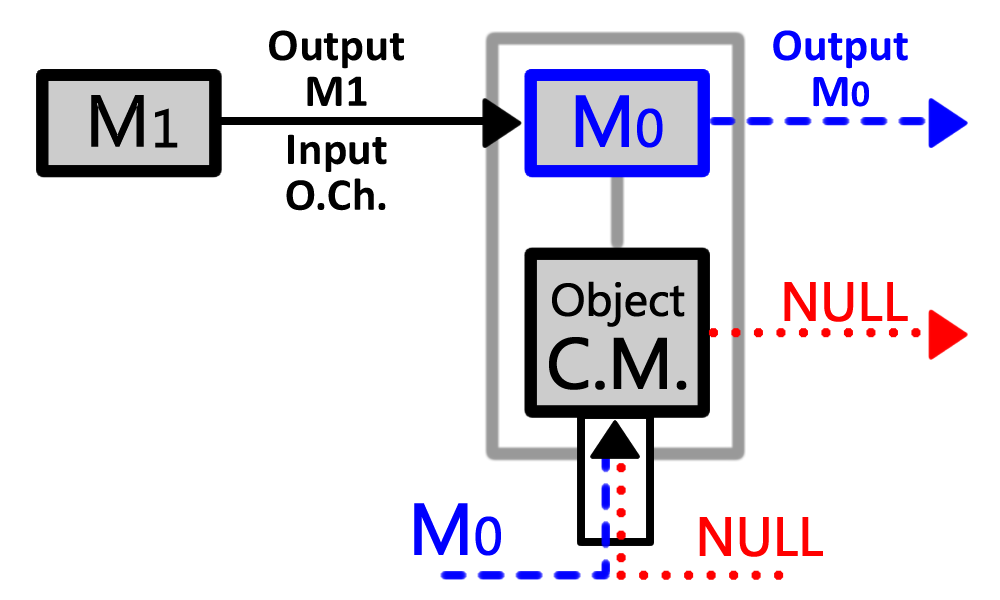
\includegraphics[width=0.4\linewidth]{O_OCh.png}
	}
	\caption[]{Communication module}
	\label{fig:och}
\end{figure}

Users can implement new computation and connection modules but \posl{} already contains many useful modules for solving a broad range of problems.

Due to the fact that \opchs{} receive information coming from outside without having control on them, it is necessary to define the {\it NULL} information, in order to denote the absence of information. If a Data Communication Module receives information, it is returned automatically. If a Object Communication Module receives a \om{}, it is instantiated and executed with the \opch's input and its result is returned. In both cases, if no available information exists (no communications performed), the \opch{} returns the {\it NULL} object.